\documentclass[12pt]{article}
\usepackage{amsmath} % AMS Math Package
\usepackage{bm}
\usepackage{amsthm} % Theorem Formatting
\usepackage{amssymb}    % Math symbols such as \mathbb
\usepackage{graphicx} % Allows for eps images
\usepackage[dvips,letterpaper,margin=1in,bottom=0.7in]{geometry}
\usepackage{tensor}
\usepackage{amsmath}
\usepackage{siunitx}
\usepackage{physics}
\usepackage{amsmath, amssymb, graphics, setspace}
\usepackage{listings}
\usepackage{color}

\definecolor{dkgreen}{rgb}{0,0.6,0}
\definecolor{gray}{rgb}{0.5,0.5,0.5}
\definecolor{mauve}{rgb}{0.58,0,0.82}

\lstset{frame=tb,
  language=Java,
  aboveskip=3mm,
  belowskip=3mm,
  showstringspaces=false,
  columns=flexible,
  basicstyle={\small\ttfamily},
  numbers=none,
  numberstyle=\tiny\color{gray},
  keywordstyle=\color{blue},
  commentstyle=\color{dkgreen},
  stringstyle=\color{mauve},
  breaklines=true,
  breakatwhitespace=true,
  tabsize=3
}

\newcommand{\mathsym}[1]{{}}
\newcommand{\unicode}[1]{{}}

\newcounter{mathematicapage}

\newtheorem{p}{Problem}
\usepackage{cancel}
\newtheorem*{lem}{Lemma}
\theoremstyle{definition}
\newtheorem*{dfn}{Definition}
 \newenvironment{s}{%\small%
        \begin{trivlist} \item \textbf{Solution}. }{%
            \hspace*{\fill} $\blacksquare$\end{trivlist}}%

\makeatletter
% we use \prefix@<level> only if it is defined
\renewcommand{\@seccntformat}[1]{%
  \ifcsname prefix@#1\endcsname
    \csname prefix@#1\endcsname
  \else
    \csname the#1\endcsname\quad
  \fi}
% define \prefix@section
\newcommand\prefix@section{}
\newcommand{\prefix@subsection}{}
\newcommand{\prefix@subsubsection}{\thesubsubsection\ - }
\renewcommand{\thesubsection}{\arabic{subsection}}
\makeatother

\begin{document}

 {\noindent\Huge\bf  \\[0.5\baselineskip] {\fontfamily{cmr}\selectfont  Project 2}         }\\[2\baselineskip] % Title
{ {\bf \fontfamily{cmr}\selectfont Quantum Mechanics}\\ {\textit{\fontfamily{cmr}\selectfont     \today}}}~~~~~~~~~~~~~~~~~~~~~~~~~~~~~~~~~~~~~~~~~~~~~~~~~~~~~~~~~~~~~~~~~~~~~~~~~~~~~    
{\large \textsc{C Seitz}
\\[1.4\baselineskip] 

For all time-dependent problems e.g., superposition states or time-dependent potentials, I use the finite difference in the time domain (FDTD) method to solve Schrodinger's equation. The algorithm is well-known, so I will just sketch the major result I use here. The idea is the break up the time-dependent Schrodinger equation into coupled differential equations for the real and imaginary parts of the wavefunction. You solve the system numerically by alternatively updating the real and imaginary wavefunctions in time.

Let $\ell\in [0,N_{x}]$ be a discrete spatial coordinate and $m,n\in[0,N_{t}]$ index time for the real $\psi_{R}(\ell)$ and imaginary $\psi_{I}(\ell)$ parts of the wavefunction, respectively. The update equations are

\begin{align*}
\frac{1}{\Delta \tau}\left(\psi_{I}^{n+1}(\ell)-\psi_{I}^{n}(\ell)\right) &= \eta\left(\psi_{R}^{m}(\ell + 1) - 2\psi_{R}^{m}(\ell)+ \psi_{R}^{m}(\ell -1 )\right) - V(\ell)\psi_{R}^{m}(\ell)
\end{align*}

\begin{align*}
\frac{1}{\Delta \tau}\left(\psi_{R}^{m+1}(\ell)-\psi_{R}^{m}(\ell)\right) &= -\eta\left(\psi_{I}^{n}(\ell + 1) - 2\psi_{I}^{n}(\ell)+ \psi_{I}^{n}(\ell -1 )\right) - V(\ell)\psi_{I}^{n}(\ell)\\
\end{align*}

where $\tau = t/\hbar$ and $\eta = \frac{\hbar^{2}}{2m\Delta x^{2}}$ (and we set $\eta=1$) is the hopping parameter. Suppose the initial state is $\ket{\alpha} = \frac{1}{\sqrt{2}}\left(\ket{0} + \ket{1}\right)$ where $\ket{0}$ and $\ket{1}$ are the ground state and first excited state for the infinite square well. Then we find the position representation $\bra{i}\ket{0}$ and $\bra{i}\ket{1}$ by solving the time-independent Schrodinger equation as in Project 1. We then can construct $\bra{i}\ket{\alpha}$, which is purely real, and assign this as the initial condition $\psi_{R}^{0}(\ell)$.

\section{Part 1}



We can work in a coordinate system centered on zero, and write

\begin{align*}
\langle x \rangle &= \sum_{a'}\sum_{a''}c_{a'}^{*}c_{a''}\bra{a'}x\ket{a''}\exp\left(\frac{-i(E_{a''}-E_{a'})t}{\hbar}\right)\\
&= \frac{1}{2}\left(\bra{0}x\ket{1}\exp\left(\frac{-i(E_{1}-E_{0})t}{\hbar}\right) + \bra{1}x\ket{0}\exp\left(\frac{-i(E_{0}-E_{1})t}{\hbar}\right)\right)\\
&= \beta \cos(\omega t)
\end{align*}

where $\beta = \bra{0}x\ket{1} = \bra{1}x\ket{0}$ (because $x$ is Hermitian) and $\omega = (E_1-E_0)/\hbar$. The angular frequency is higher for the finite square well because there is a large energy gap between the first excited state and the ground state (see the differential in the eigenvalue spectrum in Figure 1c).

\begin{figure}
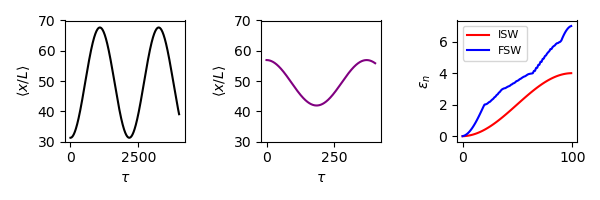
\includegraphics[scale=1]{Figure_1.png}
\centering
\caption{Expectation values of position as a function of time for the infinite (left) and finite (right) square well. Notice that both oscillate about the center of the well and the oscillation period is $\sim 10$ times longer for the infinite square well (see main text for reason)}
\end{figure}


\section{Part 2}

We are using the time-dependent Hamiltonian

\begin{align*}
H(x,t) = H_{0}(x) + \lambda(1-e^{-t/\tau})V(x)
\end{align*}

where $V(x)$ is the finite square well potential. We are assuming that $\tau\rightarrow\infty$ so the potentially turns on exactly at $t=0$, giving a constant perturbation. Notice that $V$ is going to be needed in energy basis, so we will need to transform $V$ using a unitary operator (the $\ket{i}$ basis to the $\ket{\epsilon_{n}}$ basis). 
\clearpage

Now, we are told that we start in the ground state of $H_{0}$, which is the Hamiltonian for an infinite square well, i.e. $\ket{\psi(0} = \ket{i} = \ket{1}$. recall that in time-dependent first order perturbation theory, Schrodinger's equation becomes

\begin{align*}
i\hbar\frac{d}{dt}c_{n}^{(0)}(t) &= 0\\
i\hbar\frac{d}{dt}c_{n}^{(1)}(t) &= \sum_{i}V_{ni}e^{i\omega_{ni}t}c_{i}^{(0)}(t)
\end{align*}

where $V_{ni} = \bra{n}V\ket{i}$ and $c_{n}(t)$ is the expansion coefficient for \textbf{unperturbed} energy eigenket $\ket{n}$. In general, expansion coefficients for energy eigenkets are, to first order

\begin{align*}
c_{n}(t) &\approx c_{n}^{(0)}(t) + \lambda c_{n}^{(1)}(t)\\
&= \delta_{ni} - \frac{i\lambda}{\hbar}\int_{0}^{t}V_{ni}e^{i\omega_{ni}t}dt
\end{align*}


\noindent \textbf{(H)} To first order, the transition probabilities $P(i\rightarrow n) = |c_{n}^{(1)}(t)|^{2}$ for $n=1,2,3$. From the expression above, we have

\begin{align*}
c_{n}^{(1)}(t) &= -\frac{i}{\hbar}\int_{0}^{t}V_{ni} e^{i\omega_{ni}t}dt\\
&= \frac{V_{ni}}{E_{n}-E_{i}}(1-e^{i\omega_{ni}t})
\end{align*}

Therefore,

\begin{align*}
P(i\rightarrow n) &= \frac{4|V_{ni}|^{2}}{|E_{n}-E_{i}|^{2}}\sin^{2}\left(\frac{(E_{n}-E_{i})t}{2\hbar}\right)
\end{align*}

Clearly the transition probability oscillates but the amplitude of this oscillation is small provided the magnitude of the transition matrix element $V_{ni}$ of the perturbation is small compared to the unperturbed energy difference between the initial and final states.
\clearpage

\begin{figure}
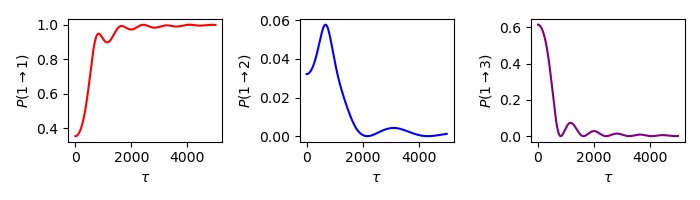
\includegraphics[scale=1]{Figure_2.png}
\centering
\caption{}
\end{figure}

\noindent \textbf{(I)} To find the wavefunction $\bra{i}\ket{\alpha(\tau)}$ analytically, recall


where the initial conditions are set such that $c_{n}(0) = \delta_{n1}$. This gives us the time-evolution of the wavefunction in the energy basis. Given all the $c_{n}(t)$'s we can consruction an energy superposition 

\begin{align*}
\ket{\beta(t)} = \sum_{n}c_{n}(t)\ket{E_{n}}
\end{align*}

So then we need to apply the unitary transformation

\begin{align*}
\ket{\beta(t)} \rightarrow U\ket{\beta(t)}
\end{align*}

to the position basis in order to obtain the wavefunction $\bra{i}\ket{\alpha(\tau)}$. To ensure we have the correct normalization we can just divide expansion coefficients by $Z = \sum_{n}|c_{n}|^{2}$.


\clearpage

\begin{figure}
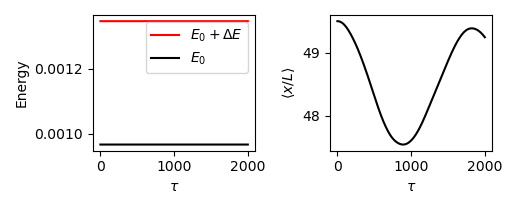
\includegraphics[scale=1]{Figure_3.png}
\centering
\caption{}
\end{figure}

\begin{lstlisting}


\end{lstlisting}

\end{document}